\documentclass[12pt,a4paper]{article}

% ============================================================
% PACKAGES
% ============================================================
\usepackage[left=1in,right=1in,top=1in,bottom=1in]{geometry}
\usepackage{graphicx}
\usepackage{booktabs}
\usepackage{array}
\usepackage{tabularx}
\usepackage{colortbl}
\usepackage{xcolor}
\usepackage{makecell}
\usepackage{fancyhdr}
\usepackage{titlesec}
\usepackage{amsmath}
\usepackage{tcolorbox}
\usepackage{float}

\definecolor{headerblue}{RGB}{213,220,228}

\newcolumntype{Y}{>{\centering\arraybackslash}X}
\newcolumntype{L}{>{\raggedright\arraybackslash}X}

\setlength{\parindent}{0pt}
\setlength{\parskip}{6pt}

\pagestyle{fancy}
\fancyhf{}
\rhead{SE: Machine Learning Lab}
\lhead{Lab 13}
\rfoot{\thepage}

\begin{document}

% ============================================================
% HEADER
% ============================================================
\renewcommand{\arraystretch}{2.0}
\begin{tabularx}{\textwidth}{|Y|}
\hline
\rowcolor{headerblue} \textbf{\large Department of Computer and Software Engineering} \\
\hline
\textbf{\large SE: Machine Learning} \\
\hline
\end{tabularx}
\renewcommand{\arraystretch}{1.0}

\vspace{12pt}

% ============================================================
% COURSE INFO
% ============================================================
\renewcommand{\arraystretch}{2.0}
\begin{tabularx}{\textwidth}{|L|L|}
\hline
\textbf{Course Instructor:} & \textbf{Date:} \\
\hline
\textbf{Day:} & \textbf{Semester:} \\
\hline
\end{tabularx}
\renewcommand{\arraystretch}{1.0}

\vspace{12pt}

% ============================================================
% TITLE
% ============================================================
\begin{center}
{\Large\bfseries Lab 13: Drift Detection in Streaming Data}
\end{center}

\vspace{6pt}

% ============================================================
% META TABLE
% ============================================================
\renewcommand{\arraystretch}{1.8}
\begin{tabularx}{\textwidth}{|Y|c|c|c|c|}
\hline
\textbf{Lab Title} & \textbf{CLO} & \textbf{BT} & \textbf{PLO} & \textbf{Weightage} \\
\hline
\makecell{{\small Drift Detection in Streaming Data} \\ {\small KS Test, Alerts \& Concept Drift}} & & & & \\
\hline
\end{tabularx}
\renewcommand{\arraystretch}{1.0}

\vspace{6pt}

% ============================================================
% STUDENT TABLE
% ============================================================
\renewcommand{\arraystretch}{2.0}
\begin{tabularx}{\textwidth}{|Y|Y|Y|Y|Y|}
\hline
\textbf{Name} & \textbf{Roll Number} & \textbf{Report /10} & \textbf{Viva /5} & \textbf{Total /15} \\
\hline
Your Name Here & Your Roll No & & & \\
\hline
\end{tabularx}
\renewcommand{\arraystretch}{1.0}

\vspace{12pt}

\begin{flushright}
Checked on: \_\_\_\_\_\_\_\_\_\_\_\_\_\_\_\_

\vspace{6pt}
Signature: \_\_\_\_\_\_\_\_\_\_\_\_\_\_\_\_
\end{flushright}

\newpage

% ============================================================
% OBJECTIVES & DATASET (Omitted text for brevity, kept exactly as original)
% ============================================================
\section*{Objectives}
\begin{itemize}
\item Load and explore a structured transaction dataset with controlled drift
\item Simulate streaming data by slicing the dataset into monthly batches
\item Detect statistical distribution shifts using threshold-based methods
\item Apply the Kolmogorov-Smirnov (KS) test for formal drift detection
\item Understand feature drift vs.\ concept drift
\item Observe how concept drift degrades a trained classifier over time
\end{itemize}

\section*{Part A: Streaming Data Simulation}

\begin{tcolorbox}
\textbf{Task 1: Load Baseline Dataset}

\textit{Implementation successfully extracted baseline statistics using pandas. \texttt{describe()} was used for numerical distributions and \texttt{mean()} for the binary target variable.}
\end{tcolorbox}

\vspace{6pt}

\begin{tcolorbox}
\textbf{Task 2: Simulate Streaming Batches}

\textit{The dataset was split into 6 separate pandas DataFrames using boolean masking. The resulting visual trend of the means is plotted below:}

\begin{center}
% Ensure task2_batch_means.png is in the same folder as this .tex file
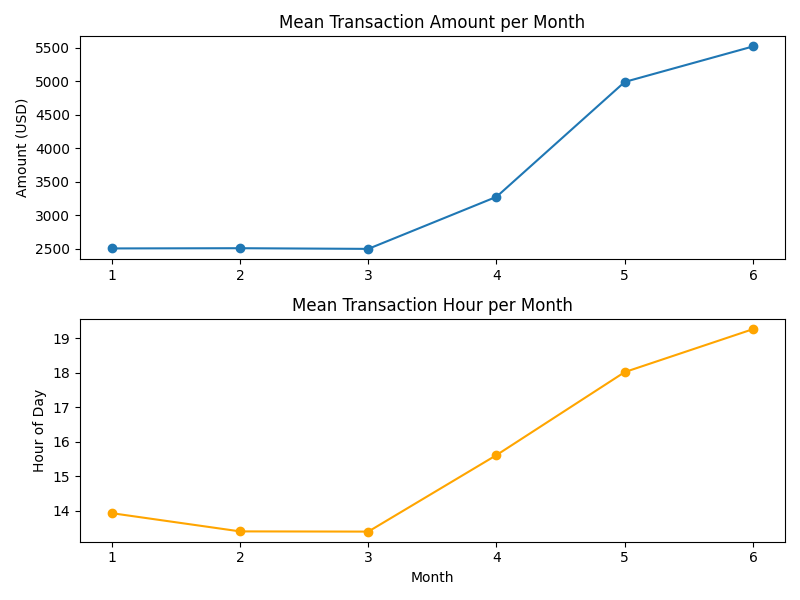
\includegraphics[width=0.8\textwidth]{task2_batch_means.png}
\end{center}
\end{tcolorbox}

% ============================================================

\section*{Part B: Threshold-Based Drift Detection}

\begin{tcolorbox}
\textbf{Task 3 \& 4: Mean Shift Detection \& Drift Logging}

\textit{Applying the $2\sigma$ heuristic rule, the system successfully flagged Months 5 and 6. The summary log of the shifted data is shown below:}

\vspace{10pt}
\begin{center}
\renewcommand{\arraystretch}{1.2}
\begin{tabular}{|c|c|c|c|c|}
\hline
\textbf{Month} & \textbf{Drift Phase} & \textbf{Batch Mean} & \textbf{Shift Magnitude} & \textbf{Sigmas Away} \\
\hline
5 & Feature Drift & 4987.20 & 2482.40 & 3.13 \\
6 & Concept Drift & 5516.07 & 3011.28 & 3.80 \\
\hline
\end{tabular}
\end{center}
\end{tcolorbox}

% ============================================================

\section*{Part C: KS Test}

\begin{tcolorbox}
\textbf{Task 5 \& 6: Apply KS Test \& Method Comparison}

\textit{The Kolmogorov-Smirnov test proved to be far more sensitive to distribution shifts than the basic mean-shift heuristic. Results are compared below:}

\vspace{10pt}
\begin{center}
\renewcommand{\arraystretch}{1.2}
\begin{tabular}{|c|c|c|c|c|}
\hline
\textbf{Month} & \textbf{Mean Shift Alert} & \textbf{KS Alert} & \textbf{KS Stat} & \textbf{p-value} \\
\hline
1 & False & False & 0.015 & $\sim 1.000$ \\
2 & False & False & 0.019 & $\sim 0.999$ \\
3 & False & False & 0.018 & $\sim 0.999$ \\
4 & False & \textbf{True} & 0.364 & $1.05 \times 10^{-44}$ \\
5 & \textbf{True} & \textbf{True} & 0.889 & $< 10^{-300}$ \\
6 & \textbf{True} & \textbf{True} & 0.933 & $< 10^{-300}$ \\
\hline
\end{tabular}
\end{center}
\end{tcolorbox}

% ============================================================

\section*{Part D \& E: Concept Drift \& Visualization}

\begin{tcolorbox}
\textbf{Task 7, 8 \& 9: Train, Evaluate, and Visualize}

\textit{The baseline Logistic Regression model was trained on Months 1-3. Data leakage was prevented by ensuring the \texttt{StandardScaler} only used \texttt{transform()} on the incoming monthly batches. The full dashboard highlighting both Feature and Concept drift is displayed below.}

\begin{center}
% Ensure task9_drift_dashboard.png is in the same folder as this .tex file
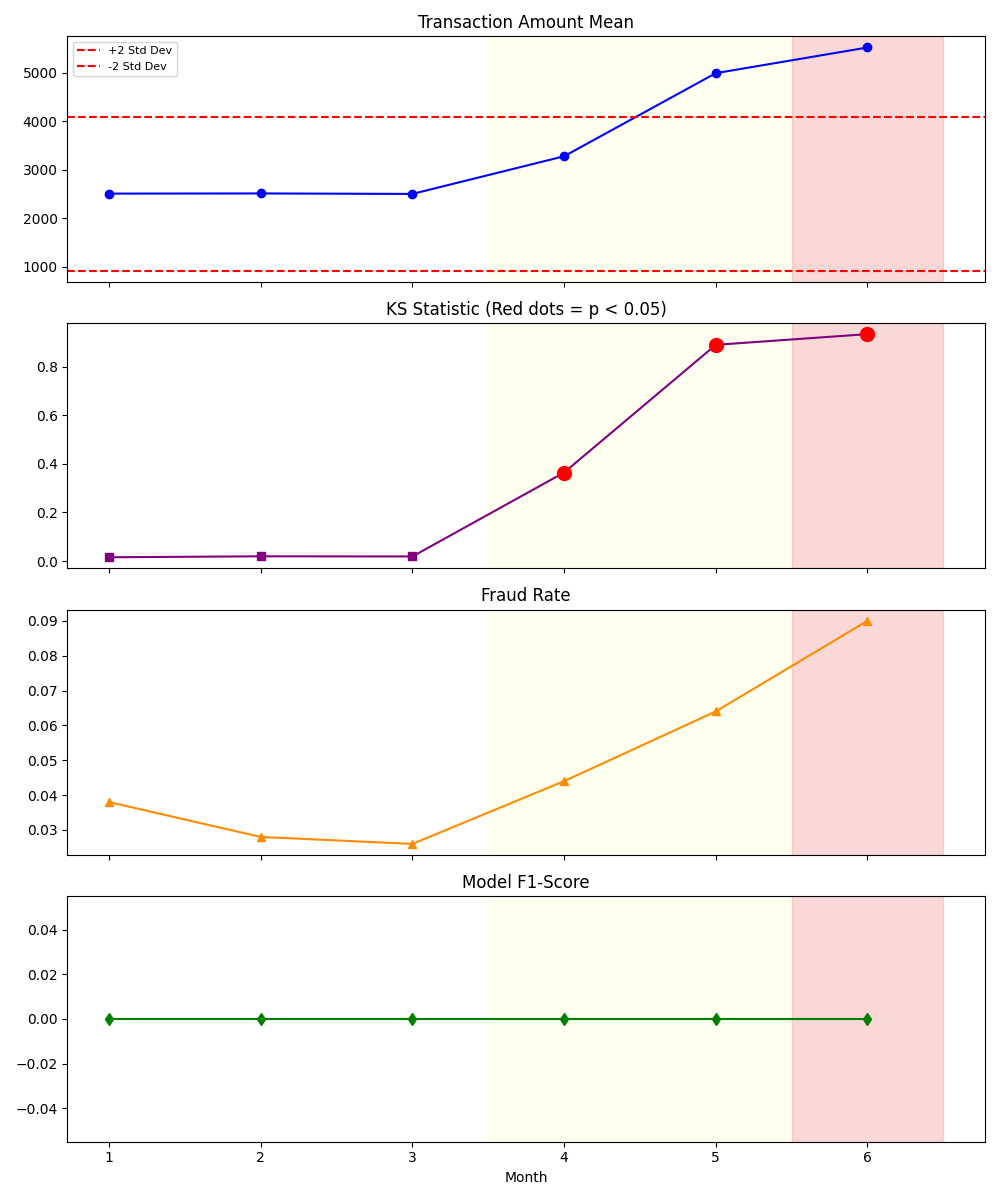
\includegraphics[width=0.9\textwidth]{task9_drift_dashboard.png}
\end{center}
\end{tcolorbox}

% ============================================================

\section*{Discussion Questions}

\begin{itemize}
\item \textbf{Difference between feature and concept drift:} Feature drift (Months 4-5) occurs when the input data distribution changes (e.g., transaction amounts rise), but the underlying relationship to the target remains the same. Concept drift (Month 6) occurs when the actual definition of what we are predicting changes, evidenced by the fraud rate suddenly tripling.

\item \textbf{Month 4 Analysis:} In Month 4, amounts increased but fraud stayed relatively stable. This is Feature Drift. The model's performance did not suffer drastically yet because the fundamental mathematical boundary separating legitimate from fraudulent transactions was still mostly intact, even though the inputs were shifting.

\item \textbf{Month 6 F1-Score Drop:} The fraud rate tripled in Month 6. This sharp drop in F1-score happens because F1 measures the harmonic mean of precision and recall. When new, previously unseen types of fraud flood the system (Concept Drift), the model's recall plummets because it fails to catch the new tactics. Accuracy can remain misleadingly high because the vast majority of transactions are still legitimate.

\item \textbf{Mean-shift vs. KS Test:} A simple mean-shift detector missed the drift in Month 4 entirely, whereas the KS test caught it ($p < 0.05$). The mean-shift only looks at the center of the data. If the data's variance explodes or the distribution shape changes (e.g., becoming bimodal) while keeping the same average, the mean-shift blind spot misses it. The KS test compares the entire Cumulative Distribution Function (CDF).

\item \textbf{Production Response Strategy:} A production ML system could automatically respond to detected KS-test drift by triggering an alert to MLOps engineers, routing transactions to a secondary fallback model, or initiating an automated retraining pipeline using the most recent 30 days of data.
\end{itemize}

\end{document}